\documentclass{beamer}

\usepackage{beamerthemesplit}
\usepackage{graphicx}
\usepackage{color, natbib, hyperref}

% define colors
\definecolor{jblue}  {RGB}{20,50,100}
\definecolor{ngreen} {RGB}{98,158,31}

%theme

\usetheme{boxes} 
%\usecolortheme{seahorse} 
\setbeamertemplate{items}[default] 
%\setbeamercovered{transparent}
\setbeamertemplate{blocks}[rounded]
\setbeamertemplate{navigation symbols}{} 
% set the basic colors
\setbeamercolor{palette primary}   {fg=black,bg=white}
\setbeamercolor{palette secondary} {fg=black,bg=white}
\setbeamercolor{palette tertiary}  {bg=jblue,fg=white}
\setbeamercolor{palette quaternary}{fg=black,bg=white}
\setbeamercolor{structure}{fg=jblue}
\setbeamercolor{titlelike}         {bg=jblue,fg=white}
\setbeamercolor{frametitle}        {bg=jblue!10,fg=jblue}
\setbeamercolor{cboxb}{fg=black,bg=jblue}
\setbeamercolor{cboxr}{fg=black,bg=red}

% reduce space before/after equations
\expandafter\def\expandafter\normalsize\expandafter{%
    \normalsize
    \setlength\abovedisplayskip{1pt}
    \setlength\belowdisplayskip{1pt}
    \setlength\abovedisplayshortskip{1pt}
    \setlength\belowdisplayshortskip{1pt}
}

% set colors for itemize/enumerate
\setbeamercolor{item}{fg=ngreen}
\setbeamercolor{item projected}{fg=white,bg=ngreen}

% set colors for blocks
\setbeamercolor{block title}{fg=ngreen,bg=white}
\setbeamercolor{block body}{fg=black,bg=jblue!10}

% set colors for alerted blocks (blocks with frame)
\setbeamercolor{block alerted title}{fg=white,bg=jblue}
\setbeamercolor{block alerted body}{fg=black,bg=jblue!10}
\setbeamercolor{block alerted title}{fg=white,bg=dblue!70} % Colors of the highlighted block titles
\setbeamercolor{block alerted body}{fg=black,bg=dblue!10} % Colors of the body of highlighted blocks

% set the fonts
\usefonttheme{professionalfonts}

\setbeamerfont{section in head/foot}{series=\bfseries}
\setbeamerfont{block title}{series=\bfseries}
\setbeamerfont{block alerted title}{series=\bfseries}
\setbeamerfont{frametitle}{series=\bfseries}
\setbeamerfont{frametitle}{size=\Large}
\setbeamerfont{block body}{series=\mdseries}
\setbeamerfont{caption}{series=\mdseries}
\setbeamerfont{headline}{series=\mdseries}


% set some beamer theme options
\setbeamertemplate{title page}[default][colsep=-4bp,rounded=true]
\setbeamertemplate{sections/subsections in toc}[square]
\setbeamertemplate{items}[circle]
\setbeamertemplate{blocks}[width=0.0]
\beamertemplatenavigationsymbolsempty

% Making a DAG
\usepackage{tkz-graph}  
\usetikzlibrary{shapes.geometric}
\tikzstyle{VertexStyle} = [shape            = ellipse,
                               minimum width    = 6ex,%
                               draw]
 \tikzstyle{EdgeStyle}   = [->,>=stealth']      


% Math macros
\newcommand{\cD}{{\mathcal D}}
\newcommand{\cF}{{\mathcal F}}
\newcommand{\todo}[1]{{\color{red}{TO DO: \sc #1}}}

\newcommand{\reals}{\mathbb{R}}
\newcommand{\integers}{\mathbb{Z}}
\newcommand{\naturals}{\mathbb{N}}
\newcommand{\rationals}{\mathbb{Q}}

\newcommand{\ind}[1]{1_{#1}} % Indicator function
\newcommand{\pr}{\mathbb{P}} % Generic probability
\newcommand{\ex}{\mathbb{E}} % Generic expectation
\newcommand{\var}{\textrm{Var}}
\newcommand{\cov}{\textrm{Cov}}

\newcommand{\normal}{N} % for normal distribution (can probably skip this)
\newcommand{\eps}{\varepsilon}
\newcommand\independent{\protect\mathpalette{\protect\independenT}{\perp}}
\def\independenT#1#2{\mathrel{\rlap{$#1#2$}\mkern2mu{#1#2}}}

\newcommand{\convd}{\stackrel{d}{\longrightarrow}} % convergence in distribution/law/measure
\newcommand{\convp}{\stackrel{P}{\longrightarrow}} % convergence in probability
\newcommand{\convas}{\stackrel{\textrm{a.s.}}{\longrightarrow}} % convergence almost surely

\newcommand{\eqd}{\stackrel{d}{=}} % equal in distribution/law/measure
\newcommand{\argmax}{\textrm{argmax}}
\newcommand{\argmin}{\textrm{argmin}}


\mode<presentation>

\title[Model-based matching]{Model-based matching for causal inference in observational studies}
\author{Kellie Ottoboni \\ with Philip B. Stark}
\institute[]{Department of Statistics, UC Berkeley\\Berkeley Institute for Data Science}
\date{March 15, 2016}

\begin{document}

\frame{\titlepage}

\AtBeginSection[]
{
   \begin{frame}
       \frametitle{Outline}
       \tableofcontents[currentsection]
   \end{frame}
}



\section[Introduction]{Introduction}
\frame
{
  \frametitle{Observational Studies vs Experiments}
 \begin{center}
\begin{itemize}
\item \textbf{Problem:} Estimate the causal effect of a treatment on outcome of interest
\item In randomized experiments, treatment is assigned to individuals at random.
\item In observational studies, the way individuals select into treatment groups is unknown.
%\item \textbf{Confounding} occurs when a variable affects both treatment assignment and the outcome. It biases our estimates of the treatment effect.
\end{itemize}

\begin{figure}[h]
\begin{tikzpicture}
\SetGraphUnit{2} 
\Vertex{Outcome} \NOWE(Outcome){Treatment} \NOEA(Outcome){Confounder}
\Edges[color=red, label=?](Treatment, Outcome) \Edges(Confounder, Outcome) \pause \Edges(Confounder, Treatment) 
\end{tikzpicture}
\end{figure}
\end{center}
}





\frame{
\frametitle{Neyman-Rubin Causal Model}
\begin{center}
\begin{itemize}
\item Population of $i = 1, \dots, N$ individuals. Each individual has two \textbf{potential outcomes}.
\item $Y_i(1)$ is individual $i$'s outcome if he receives treatment
\item $Y_i(0)$ is individual $i$'s outcome if he is in the control group
\item The treatment effect for individual $i$ is $\tau_i = Y_i(1) - Y_i(0)$
\end{itemize}
\vfill
\begin{tikzpicture}
\draw (0,0) rectangle (1,1) node[pos=.5] {$Y_2(1)$};\draw (1,0) rectangle (2,1)node[pos=.5] {$Y_2(0)$};
\draw (0,1.5) rectangle (1,2.5) node[pos=.5] {$Y_1(1)$}; \draw (1,1.5) rectangle (2,2.5) node[pos=.5] {$Y_1(0)$};
\draw (3,0) rectangle (4,1) node[pos=.5] {$Y_4(1)$}; \draw (4,0) rectangle (5,1) node[pos=.5] {$Y_4(0)$};
\draw (3,1.5) rectangle (4,2.5) node[pos=.5] {$Y_3(1)$}; \draw (4,1.5) rectangle (5,2.5) node[pos=.5] {$Y_3(0)$};
\end{tikzpicture}

\end{center}
}

\frame{
\frametitle{Fundamental Problem of Causal Inference \small{\citep{holland_statistics_1986}}}
\begin{center}
\begin{itemize}
\item We may never observe both $Y_i(1)$ and $Y_i(0)$
\item $T_i$ is a treatment indicator: $1$ if $i$ is treated, $0$ if $i$ is control
\item The observed outcome for individual $i$ is $Y_i = T_iY_i(1) + (1-T_i)Y_i(0)$
\end{itemize}

\vfill
\begin{tikzpicture}
\draw (0,0) rectangle (1,1) node[pos=.5] {$Y_2(1)$}; \draw[fill=black]  (1,0) rectangle (2,1)node[pos=.5] {$Y_2(0)$};
\draw (0,1.5) rectangle (1,2.5) node[pos=.5] {$Y_1(1)$}; \draw[fill=black]  (1,1.5) rectangle (2,2.5) node[pos=.5] {$Y_1(0)$};
\draw[fill=black]  (3,0) rectangle (4,1) node[pos=.5] {$Y_4(1)$}; \draw (4,0) rectangle (5,1) node[pos=.5] {$Y_4(0)$};
\draw[fill=black]  (3,1.5) rectangle (4,2.5) node[pos=.5] {$Y_3(1)$}; \draw (4,1.5) rectangle (5,2.5) node[pos=.5] {$Y_3(0)$};
\end{tikzpicture}
\end{center}
}


\frame{
\frametitle{Estimands}
\begin{center}
\begin{itemize}
\item Average treatment effect
$$\mathbb{E}( Y_i(1) - Y_i(0))$$
\item Average treatment effect on the treated
$$\mathbb{E}(Y_i(1) - Y_i(0) \mid T_i = 1)$$
\item Conditional average treatment effect
$$ \mathbb{E}(Y_i(1) - Y_i(0) \mid X_i) $$
\item If treatment effect varies by covariates $X$, then averages might not be informative
\end{itemize}
\end{center}
}

\section[Matching]{Matching}

\frame
{
\frametitle{Matching}
\begin{center}
How can we estimate the counterfactual for treated individuals? \\
\vfill
\begin{itemize}
\item \textbf{Ideal:} group individuals by $X_i$ to estimate subgroup treatment effects and then average over subgroups
\item \textbf{Reality:} many covariates, perhaps continuous, make it difficult to stratify
\end{itemize}
	

\begin{tikzpicture}[scale = 0.5]
\foreach \x in{0,...,4}
{   \draw (0,\x ,4) -- (4,\x ,4);
    \draw (\x ,0,4) -- (\x ,4,4);
    \draw (4,\x ,4) -- (4,\x ,0);
    \draw (\x ,4,4) -- (\x ,4,0);
    \draw (4,0,\x ) -- (4,4,\x );
    \draw (0,4,\x ) -- (4,4,\x );
}
\end{tikzpicture}
\end{center}
}



\frame
{
\frametitle{Aside... the curse of dimensionality }
\begin{center}
\vfill
\begin{itemize}
\item If $d$ covariates are split into $k$ bins, we have $d^k$ groups.
\item To guarantee that we have at least one treated and one control in each group with $95\%$ probability, we need
$$n \geq \frac{2 \log(1 - (0.95)^{1/k^{d+1}})}{\log(\frac{k^d - 1}{k^d})}$$
\item If $d = 5$ and $k = 2$, $n \geq 225$.\\
\item If $d = 10$ and $k = 2$, $n \geq 10,844$.
\end{itemize}
\end{center}

\begin{flushright}
\begin{tikzpicture}[scale = 0.5, remember picture]
\foreach \x in{0,...,4}
{   \draw (0,\x ,4) -- (4,\x ,4);
    \draw (\x ,0,4) -- (\x ,4,4);
    \draw (4,\x ,4) -- (4,\x ,0);
    \draw (\x ,4,4) -- (\x ,4,0);
    \draw (4,0,\x ) -- (4,4,\x );
    \draw (0,4,\x ) -- (4,4,\x );
}
\end{tikzpicture}
\end{flushright}

}
	

\frame{
\frametitle{Matching}
\begin{center}
\begin{itemize}
\item \textbf{Solution:} use a one-dimensional score to match or group individuals
\end{itemize}
\end{center}
}


\subsection[Propensity score matching]{Propensity score matching}

\frame{
\frametitle{Propensity score matching}
\begin{itemize}
\item The \textbf{propensity score} is an individual's probability of being assigned treatment, conditional on their covariates
$$ p(x) = \mathbb{P}(T = 1 \mid X = x)$$
\item The propensity score is a balancing score: $X \independent T \mid p(X)$
\item For individuals with the same propensity score, treatment assignment is as if random
\end{itemize}
}

\frame{
\frametitle{Propensity score matching}
\begin{theorem}[\cite{rosenbaum_central_1983}]
If treatment assignment is independent of potential outcomes given $X$, 
$$(Y(1), Y(0)) \independent T \mid X$$
 and if every unit has a chance of receiving treatment,
 $$0 < p(X) < 1 \text{ for all }X$$
 then $(Y(1), Y(0)) \independent T \mid p(X)$.
\end{theorem}
In particular, treated units can serve as the counterfactual for controls with the same $p(X)$ 

$$\ex(Y(t) \mid T=1, p(X)) = \ex(Y(t) \mid T=0, p(X)) \text{ for } t = 0,1$$
}

\frame{
\frametitle{Propensity score matching}
\begin{center}
This result identifies the average treatment effect in terms of quantities we can estimate:

\begin{align*}
 \ex(Y(1) - Y(0)) &= \ex_{p(x)}\left[ \ex(Y(1) - Y(0) \mid p(x) ) \right] \\
&= \ex_{p(x)}\left[ \ex(Y(1) \mid p(x) ) - \ex(Y(0) \mid p(x) ) \right] \\
&= \ex_{p(x)}\left[ \ex(Y \mid p(x), T=1 )  -\ex(Y \mid p(x), T=0 ) \right] \\
\end{align*}
\end{center}
}


%\frame{
%\frametitle{Propensity score matching}
%How to use the result to estimate the average treatment effect?
%\begin{itemize}
%\item Often, the true propensity score is unknown. Estimate $\hat{p}(x)$ using logistic or probit regression
%\item Match or stratify units on $\hat{p}(x)$
%\item Within groups, take difference in mean outcomes between treated and controls
%\item Average estimated treatment effects across groups
%\end{itemize}
%}


\frame{
\frametitle{Propensity score matching}
$p(x)$ is usually unknown and estimated by $\hat{p}(x)$ using logistic or probit regressions
\begin{itemize}
\item Assumes a simple functional form for relationship between covariates and treatment
\item Assumes that probability of treatment takes same form for all individuals
\item May actually worsen balance if estimated incorrectly \citep{diamond_genetic_2012}
\end{itemize}
\vfill
Matching introduces bias
\begin{itemize}
\item Standard errors are difficult to compute for matching estimators \citep{abadie_large_2006, abadie_failure_2008}
\item There's no ``optimal'' way to match
\end{itemize}

}


\subsection[Model-based Matching]{Model-based Matching}

\frame{
\frametitle{Model-based Matching}
\textbf{Idea:} Instead of modeling the propensity score, model the outcome \\
\vfill
Stratify on $\hat{Y}$, the ``best'' prediction of the outcome based on all covariates except for the treatment
}


\frame
{
  \frametitle{Model-based Matching}
\begin{center}
\begin{itemize}
\item Under standard assumptions (conditional independence of treatment and potential outcomes given $X$), the \textbf{average treatment effect} is nonparametrically identified
\item Estimate it using the difference in average residuals, $Y - \hat{Y}$, between treated and controls
\end{itemize}

\begin{figure}[htbp]
\begin{center}
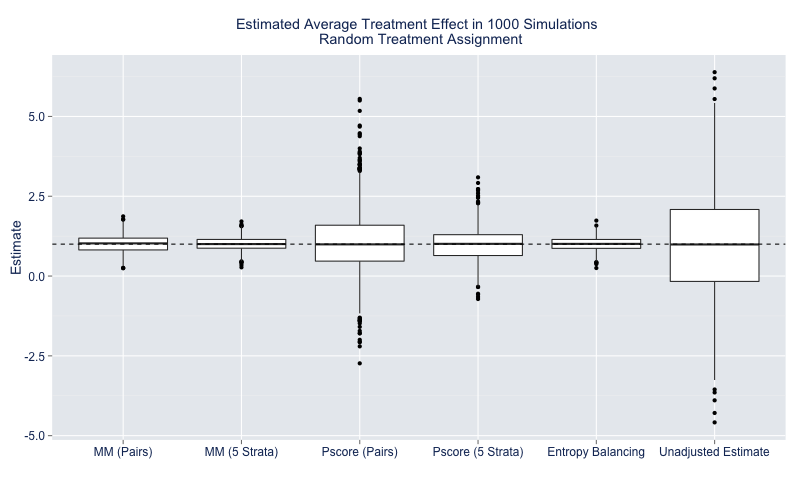
\includegraphics[width = 0.9\textwidth]{fig/estimates.png}

\end{center}
\end{figure}


\end{center}
}

\frame
{
  \frametitle{Model-based Matching}
\begin{center}
\begin{itemize}
\item Use stratified permutation test to test the \textbf{strong null hypothesis} of no treatment effect whatsoever
\item Stratifying on $\hat{Y}$ allows us to detect non-constant and non-linear treatment effects
\end{itemize}

\begin{figure}[htbp]
\begin{center}
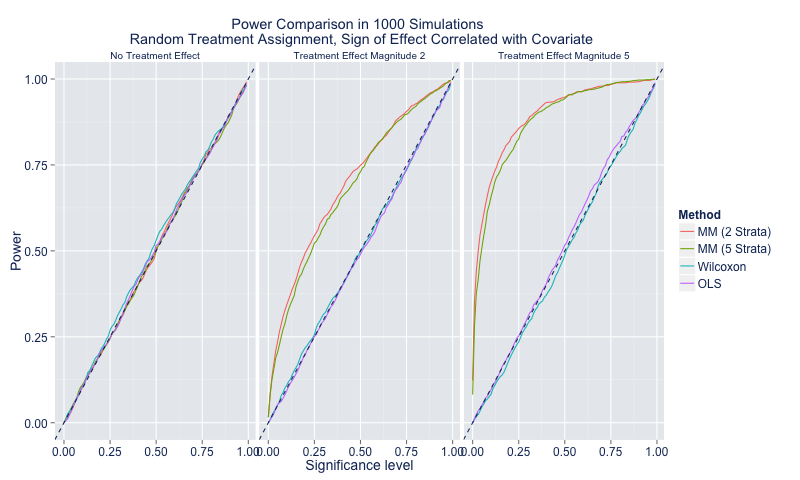
\includegraphics[width = 0.9\textwidth]{fig/power.png}
\end{center}
\end{figure}


\end{center}
}

\section[Examples]{Examples}

\subsection[Toads and Packstock in Yosemite]{Toads and Packstock in Yosemite}

\frame{
\frametitle{Salt}
\begin{center}
\begin{figure}[htbp]
\begin{center}
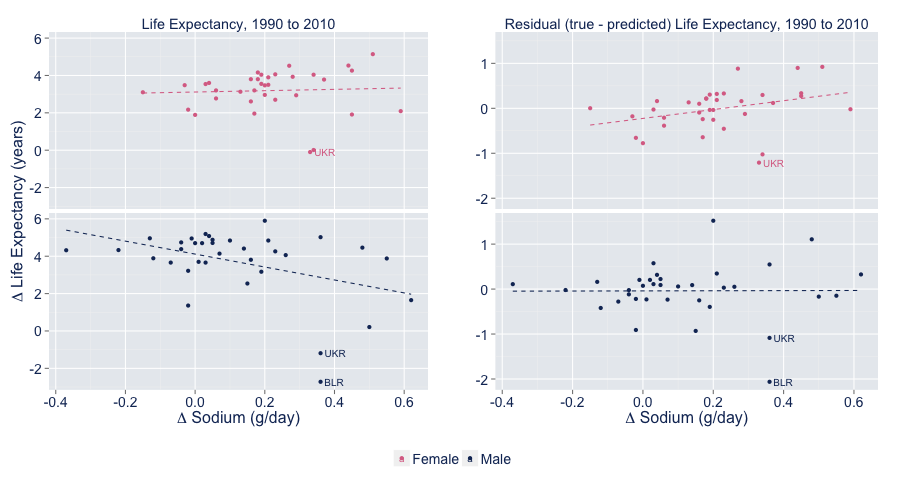
\includegraphics[width = 0.9\textwidth]{fig/sodium_lifeexp.png}
\end{center}
\end{figure}
\end{center}
}

\subsection[Salt and Mortality]{Salt and Mortality}

\section[Conclusions]{Conclusions}
\frame
{
  \frametitle{Future Directions}
\begin{center}
\begin{itemize}
\item Do different test statistics give greater power when the treatment effect is nonlinear?
\item What is the optimal way to stratify?
\item How to quantify uncertainty -- standard errors and confidence intervals?
\end{itemize}
\end{center}
}




\section{References}
\begin{frame}
\frametitle{References}
\bibliographystyle{plainnat}
\bibliography{refs}
\itemize
\end{frame}

\end{document}
